\documentclass{beamer}
\usepackage[utf8]{inputenc}
\usepackage[T1]{fontenc} 
\usetheme{Luebeck}
\setbeamercovered{transparent}

\title[Izgradnja 3D modela scene pomoću 3D kamere]{Izgradnja 3D modela
scene pomoću 3D kamere}
\author{Marijan Svalina}
\institute{Elektrotehnički fakultet Osijek \\ Diplomski studij
računarstva}
\date{Srpanj, 2014}
\begin{document}

\begin{frame}
    \titlepage
\end{frame}


\begin{frame}{Pregled prezentacije}
    \tableofcontents[pausesections]
\end{frame}

% Prije pregleda zadatka rada govoriti ću o tehnologiji i zajednici koja
% je omogućila postojanje ovog rada.

\section{Uvod} 
\begin{frame}{Uvod, priznanja i temelji rada}
    \minipage{0.38\textwidth}
        \includegraphics<1->[width=\linewidth]{../figures/kinect2.png}
    \endminipage
    \minipage{0.32\textwidth}
        \includegraphics<2->[width=\linewidth]{../figures/gpl.png}
    \endminipage
    \minipage{0.26\textwidth}%
        \includegraphics<3->[width=\linewidth]{../figures/bsd.png}
    \endminipage
\end{frame}

\subsection{Zadatak i opis projekta}
\begin{frame}{Grafički prikaz zadatka projekta}
    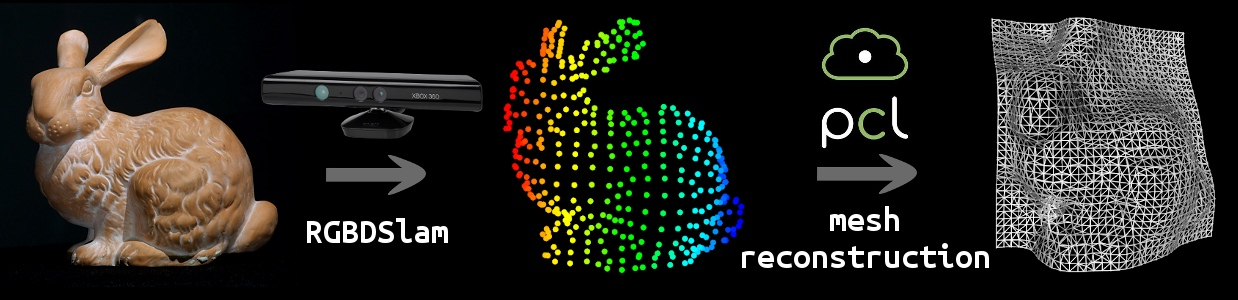
\includegraphics[width=\linewidth]{../figures/project-description.jpeg}
\end{frame}


\section{Pregled upotrebljenih tehnologija i algoritama} 
\begin{frame}
    \tableofcontents[currentsection]
\end{frame}

\subsection{Microsoft Kinect kamera}
\begin{frame}{Kinect 3D kamera}
    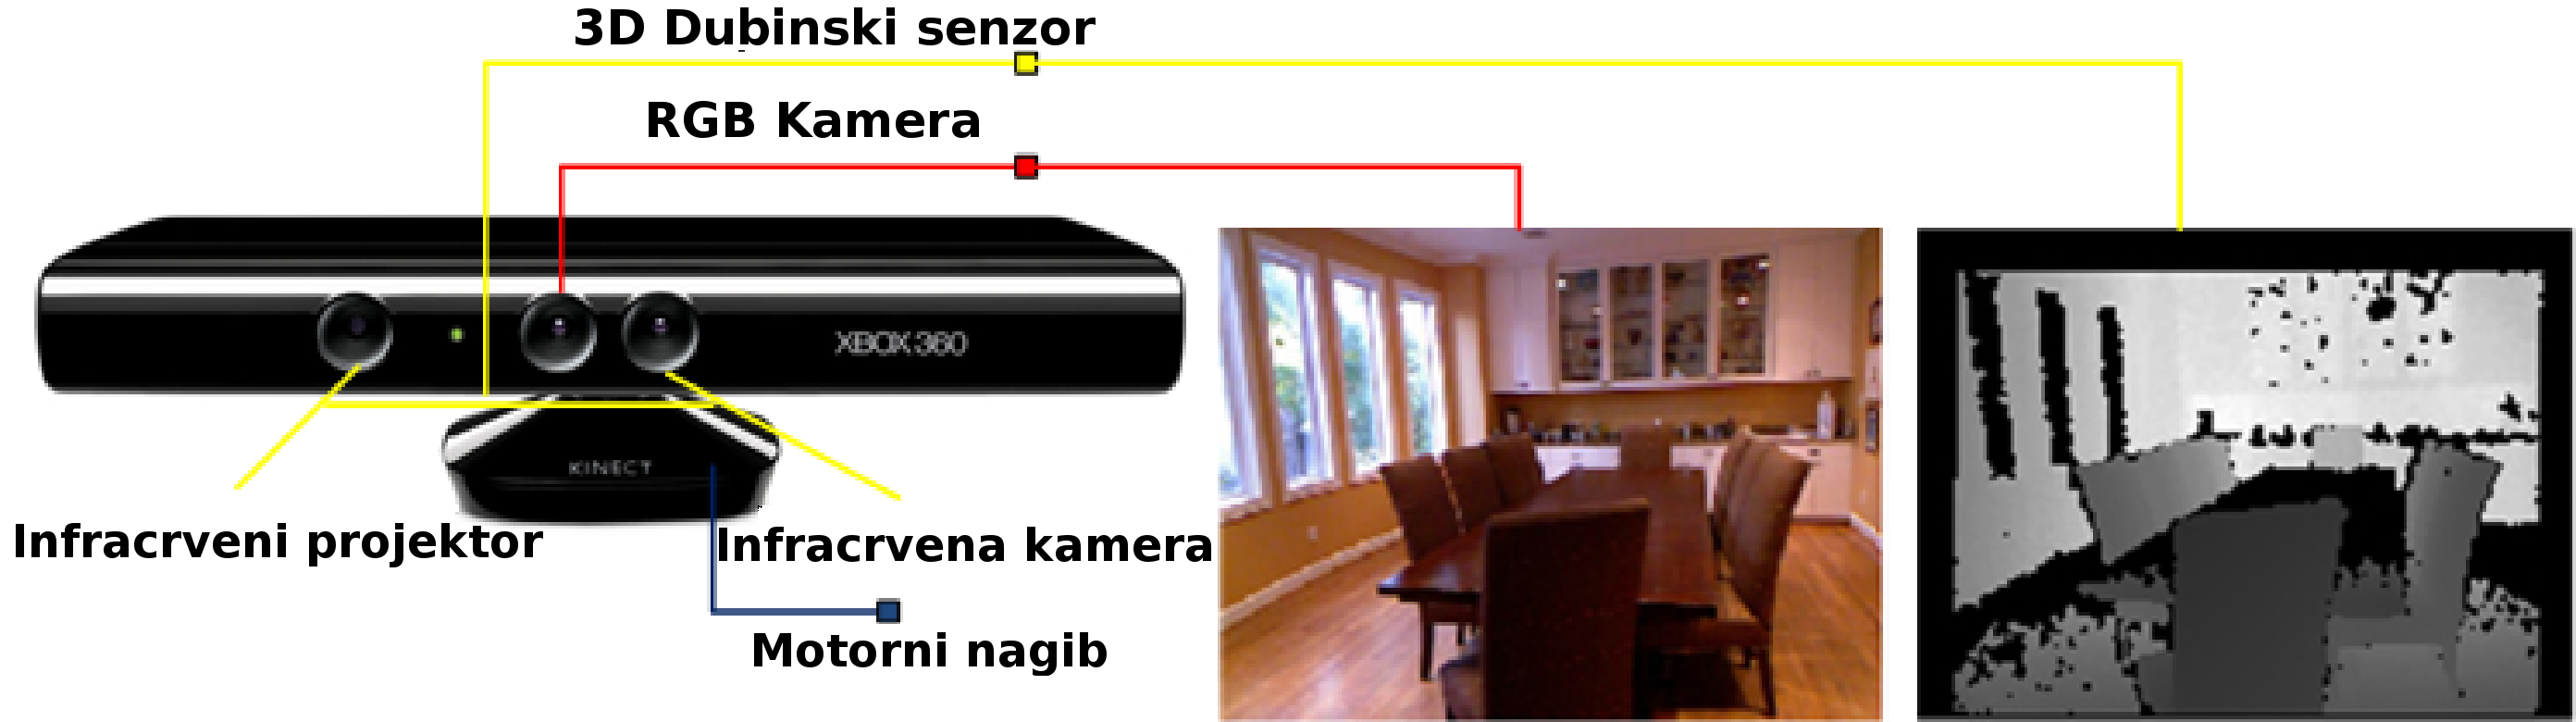
\includegraphics[width=\linewidth]{../figures/kinect.png}
\end{frame}

\begin{frame}{Kinect 3D kamera - princip rada strukturirane svjetlosti}
    \begin{itemize}
        \item <1-> IR projektor projicira \alert{jedinstven} uzorak točkastih mrlja.
        \item <2-> IR kamera hvata reflektirane IR mrlje.
        \item <3-> Geometrijska veza ostvaruje se offline kalibracijskom
            procedurom
    \end{itemize}
    
\end{frame}

\subsection{ROS biblioteka i alati}
\begin{frame}{ROS - Operacijski sustav za robote}
    
\end{frame}

\subsection{PointCloud biblioteka}
\begin{frame}{Biblioteka funkcija i algoritama za rad s oblakom
    točaka}
    
\end{frame}

\subsection{Istovremena lokalizacija i mapiranje}
\begin{frame}{Izgradnja karte nepoznatne okoline i istovremena
    navigacije upotrebom te karte}
    
\end{frame}

\subsection{Poisson algoritam za rekonstrukciju površine}
\begin{frame}{Poisson algoritam za rekonstrukciju površine - osnovna
    ideja}
    
\end{frame}

\section{Snimanje i izgradnja 3D modela scene} 
\subsection{Snimanje scene RGBDSlam programom} 
\begin{frame}{Opis rada RGBDSlam programa}

\end{frame}

\subsection{Izgradnja 3D modela scene pomoću mreže trokuta} 
\begin{frame}{Pregled razvijenog programa mesh-reconstruction}
    
\end{frame}

\section{Rezultati pokusa} 
\subsection{Prikaz izgrađenih modela scena i objekata}
\begin{frame}{Ispitivanje funkcionalnosti snimanjem nekoliko scena}

\end{frame}

\section{Zaključak} 
\begin{frame}{Prednosti, nedostatci, budućnost}

\end{frame}
\end{document}
